\documentclass[11pt]{article}
\usepackage[hmargin=1in,vmargin=1in]{geometry}
\usepackage{xcolor}
\usepackage{amsmath,amssymb,amsfonts,url,sectsty,framed,tcolorbox,framed}
\usepackage{multicol}
\setlength{\columnsep}{0.5cm}
\usepackage{blindtext}
\usepackage{amsmath}
\usepackage{cancel}

\newcommand{\pf}{{\bf Proof: }}
\newtheorem{theorem}{Theorem}
\newtheorem{lemma}{Lemma}
\newtheorem{proposition}{Proposition}
\newtheorem{definition}{Definition}
\newtheorem{remark}{Remark}
\newtheorem{th1}{}

\newcommand{\qed}{\hfill \rule{2mm}{2mm}}


\begin{document}
%%%%%%%%%%%%%%%%%%%%%%%%%%%%%%%%%%%%%%%%%%%%%%%%%%%%%%%%%%%%%%%%%%%%%

\noindent
\rule{\textwidth}{1pt}
\begin{center}
{\bf [CS304] Introduction to Cryptography and Network Security}
\end{center}
Course Instructor: Dr. Dibyendu Roy \hfill Winter 2022-2023\\
Scribed by: Rathva Kaushikkumar Sanjaybhai (202051156) \hfill Week : 3 (5-6th lecture \#)
\\
\rule{\textwidth}{1pt}

%%%%%%%%%%%%%%%%%%%%%%%%%%%%%%%%%%%%%%%%%%%%%%%%%%%%%%%%%%%
%write here
\section{OTP(One time padding):}
OTP provides perfect secrecy under some condition.

\subsection{Encryption :}
$P\ \rightarrow\ $ plain text\\
$K\ \rightarrow\ $ Secret key\\

$Enc(P,k)\ =\ p \oplus k =\ C$

\subsection{decryption :}

$Dec(C,k)\ =\ C \oplus k =\ CP$\\

$P_r[message | Cipher text] = P_r[message]$

\subsection{Conditions for it to have perfect secrecy:}
\begin{enumerate}
    \item The secret key k can't be used to encrypt the message.
    \item length(k) $\ge$ length(p)
    \item k is uniformly selected from any space.
\end{enumerate}

\section{OTP on one bit of message :}
message $\rightarrow\ m\ \epsilon\ \{0,1\}\hspace{2.5cm}$ where, key k $\epsilon\ \{0,1\}$ \\

$P_r[m=0]\ =\ P\hspace{4cm} P_r[k=0]=0.5 $\\

$P_r[m=1]\ =\ 1-P\hspace{3.5cm} P_r[k=1]=0.5 $\\

\newpage
\subsection{Encryption :}
$C\ =\ m\ \bigoplus\ k$\\\\
for cipher text to be 0 :\\
either m = k = 0 or m = k = 1 are 2 possibilities.

So ,\\  
$\begin{aligned}
P[C=0]\ &= \ P_r[m=0,k=0]\ +\ P_r[m=1,k=1]\\
 &=\ P_r[m=0]\cdot P_r[k=0]\ +\ P_r[m=1]\cdot P_r[k=1]\\
 &=\ P\times(0.5)\ +\ (1-P)\times0.5 \\\\
\end{aligned}$
 
 similar can be proven for C = 1.\\
 
 $P_r[M=m|C=c] = P_r[M=m]$\\
\begin{enumerate}
    \item $P_r(A/B)\ =\ \frac{P_r(AB)}{P_r(B)}$
    \item $P_r(AB)\ =\ P_r(B/A) \cdot P(A) $ \\
\end{enumerate}

\subsection{Perfect secrecy of OTP:}
$\begin{aligned}
P_r[M=0 | C=0] & = \frac{P_r[M=0,C=0]}{P_r[C=0]} \hspace{2.5cm} \\\\
& P_r[M=0,C=0]\ =\ \text{Probability of M and C being 0.} \\\\
& = \frac{P_r[C=0|M=0] \times P_r[M=0]}{1/2} \\\\
& \text{ Here,We are assuming that } P_r[C=0|M=0]\ =\  \text{0.5.} \\\\
& = \frac{ \bcancel{1/2} \times P_r[M=0]}{ \bcancel{1/2}}\\
& = P_r[M=0]\\\\
\end{aligned}$

C depends on k and M given m=0 k can be 1 or 0.\\

$P_r[M=0|C=0]\ =\ P_r[M=0]\ $ So it provides perfect secrecy.

\newpage

\subsection{OTP with out Condition :}
\begin{enumerate}
    \item Reuse secret key.\\
    
    $\begin{aligned}
    M_1 \bigoplus k = C_1\\
    M_2 \bigoplus k = C_2\\\\
    \end{aligned}$
    
    $\begin{aligned}
    C_1 \bigoplus C_2 & = (M_1 \bigoplus k) \bigoplus (M_2 \bigoplus k) \\
    & = M_1 \bigoplus M_2 \\
    \end{aligned}\\$

    So the xor of cipher texts will give diffrence between cipher text and message/plain text.\\

    
    \item length of key $\ge$ length of plain text.\\
    let's suppose len(k) $<$ len(P)\\
    
    $C\ =\ P\ \bigoplus \ k$ \\
    
    $
    \begin{aligned}
    & P\ =\ p_1\ p_2\ .\ .\ .\ .\ p_l\ p_{l+1}\ .\ .\ .\ p_n\ \\ 
    \bigoplus \quad & k\ =\ k_1\ k_2\ .\ .\ .\ .\ k_l\ k_1\ .\ .\ .\ k_t \\\\
    \end{aligned}$

    \hrule

    $C\ =\ (p_1 \bigoplus k_1) (p_2 \bigoplus k_2) .\ .\ .\ (p_l \bigoplus k_l)(p_{l+1} \bigoplus k_1) .\ .\ .\ (p_n \bigoplus k_t)$\\
    

    \item If we take k from a non-uniformly.The $P_r[C=0|M=0]$ will not be 0.5.\\
    So $P_r[M=0|C=0]\ \text{will not be equal to} \ P_r[M=0]\ $ and OTP will not have perfect secrecy.
\end{enumerate}

\newpage

\section{Data Encryption Standard (DES): }
- It's a block cipher Designed by IBM in 1970s and was proprietary until 1977.

\textbf{Characteristics of DES :}
\begin{enumerate}
    \item Block size = 64 bit.
    \item Number of rounds = 16
    \item Secret key size = 64 bit \\
    Out of 64 key consists of 56 bit actual key and 8 bit parity bits.
    \item It's based on Feistel Network.\\\\
\end{enumerate}

\begin{multicols}{2}
\subsection{Encryption :}
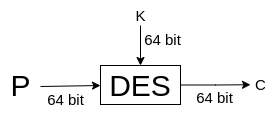
\includegraphics{Images/L_5-6/DES-Enc-Dec.drawio.png}
\columnbreak
\subsection{decryption :}
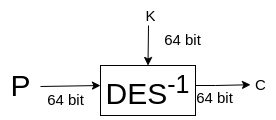
\includegraphics[scale=0.95]{Images/L_5-6/DES-Enc-Dec.drawio (1).png}
\end{multicols}
\subsection{Parity Check :}
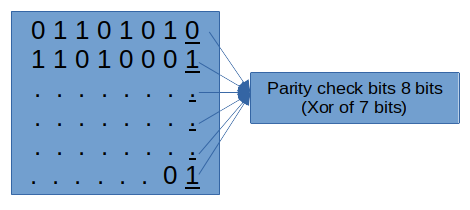
\includegraphics{Images/L_5-6/Parity Check.png}\\
After discarding 8 parity bits we have Secret key of length 58 bits.\\
In DES 16 round keys $k_1-k_{16}$are generated by key scheduling function G(n) which takes secret key as input. 

\newpage

\section{Structure of DES : }
\subsection{Encryption :}
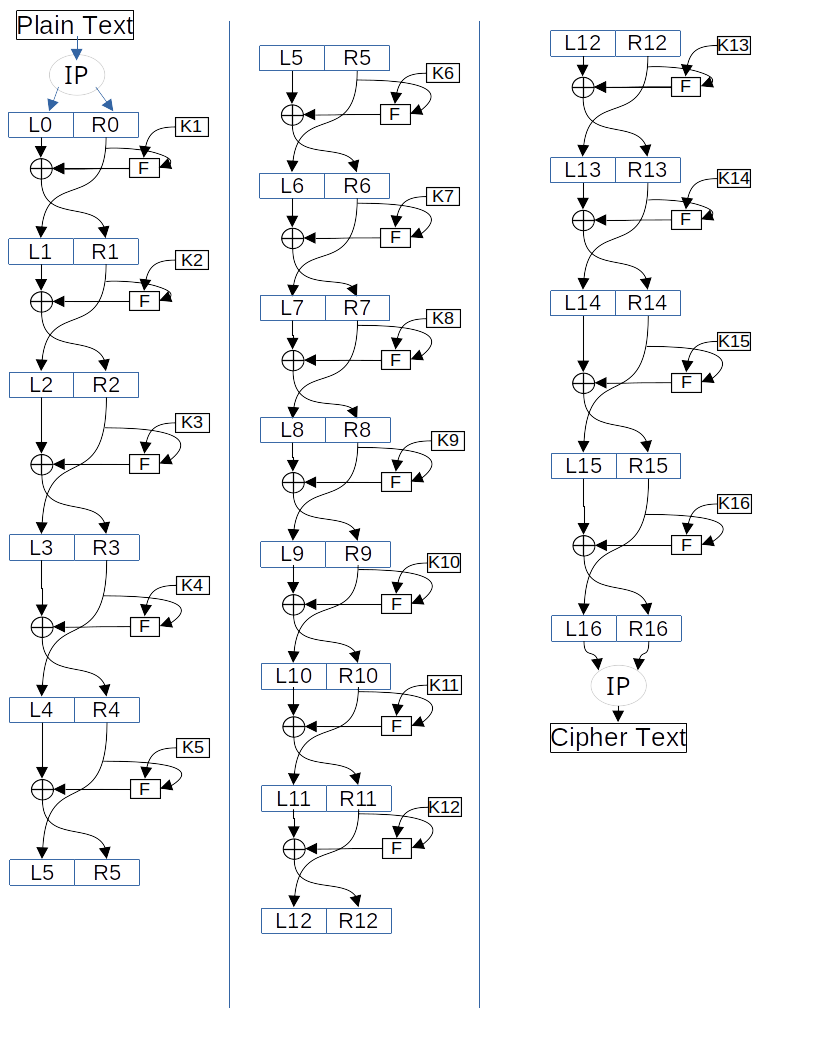
\includegraphics[scale=0.6]{Images/L_5-6/DES Structure.png}
\newpage
\subsection{Decryption :}
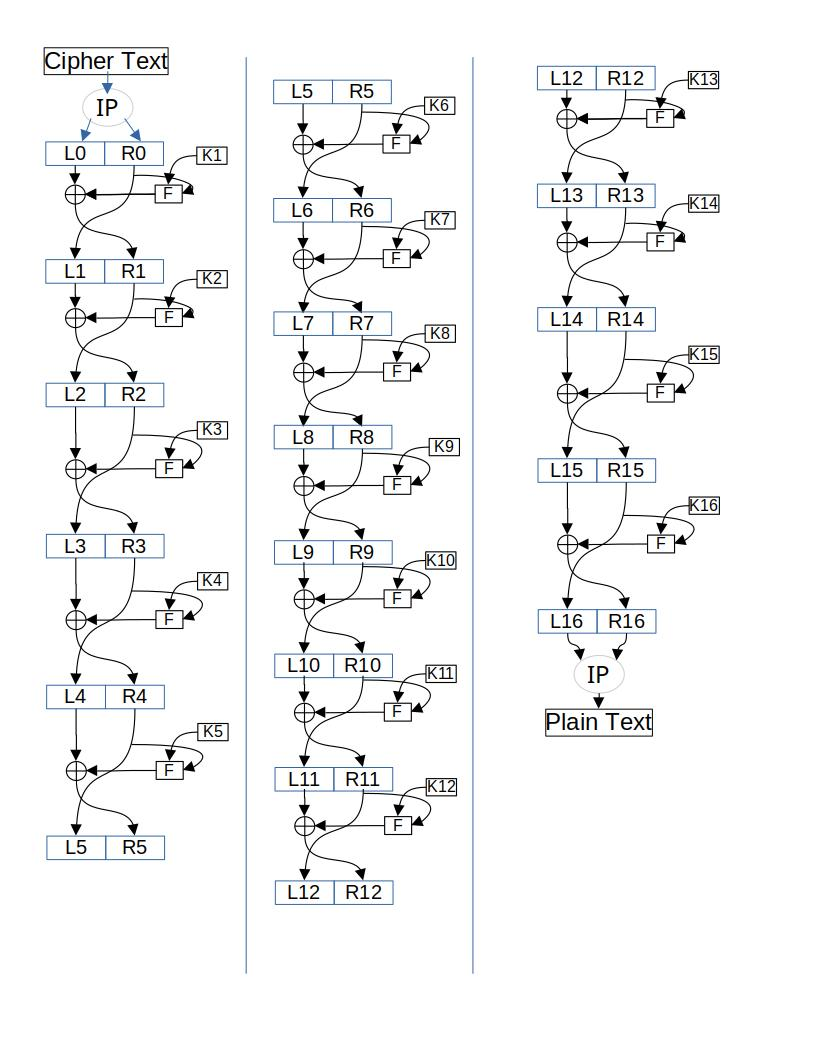
\includegraphics[scale=0.8]{Images/L_5-6/DES Structure-Dec.jpg}
\newpage
\subsection{IP (Initial Permutation):}

IP : $\{0,1\}^{64} \rightarrow \{0,1\}^{64}$
\begin{multicols}{2}
\textbf{IP lookup table}\\

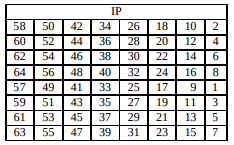
\includegraphics{Images/L_5-6/IP.png}\\
IP\((m_1m_2\ .\ .\ .\ m_{64})\ =\ (m_58m_50\ .\ .\ .\ m_15 m_7)\)    

\columnbreak
\textbf{$IP^{-1}$ lookup table}\\\\
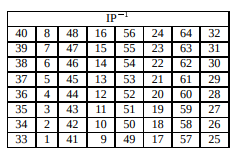
\includegraphics{Images/L_5-6/IP_INV.png}\\
\(IP^{-1}(m_1m_2\ .\ .\ .\ m_{64})\ =\ (m_40m_8\ .\ .\ .\ m_57 m_25)\)    
\end{multicols}

\subsection{Round function of DES :}

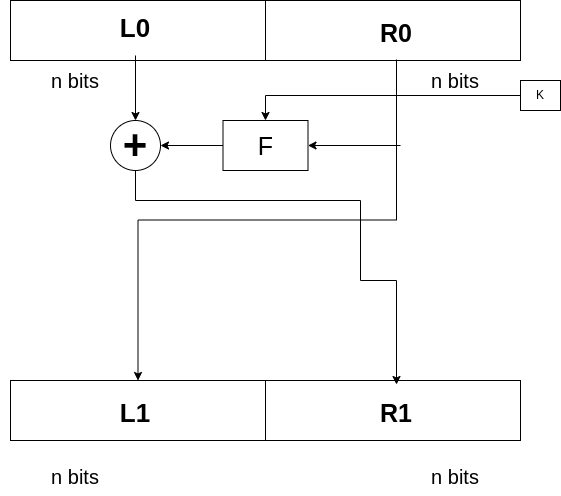
\includegraphics[scale=0.35]{Images/L4/L4_Cryupto_FN.drawio.png}\\
$f : \{0,1\}^{32} \times \{0,1\}^{48} \rightarrow \{0,1\}^{32}$\\
$f:(R_i,k_i)\ =\ X_i$\\
where,
$R_i$ is 32 bit.\\
$k_i$ is 48 bit.\\
$X_i$ is 32 bit.\\

$ f(R_i,k_i) = P(S(E(R_i) \bigoplus k_i))$\\\\
where,
$E : Expenion function : \{0,1\}^{32} \rightarrow \{0,1\}^{48}$\\
$S : Sbox : \{0,1\}^{48} \rightarrow \{0,1\}^{32} $\\
$P : Permutation : \{0,1\}^{32} \rightarrow \{0,1\}^{32}$\\\\

\newpage
\begin{multicols}{2}
\subsection{Expansion function :}
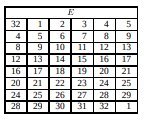
\includegraphics[scale=1.6]{Images/L_5-6/ExpansionFunction.png}\\   
$E(x_1 x_2 .\ .\ .\ x_{32}) \\ =\ \{ x_{32}\ x_1\ .\ .\ .\ x_4\ x_5\ .\ .\ .\ x_{32}\ x_1\ \}$\\

\columnbreak

\subsection{Sbox :}
S(x) = y, where x is 48 bit and y is 32 bit.\\
$X = B_1\ B_2\ B_3\ B_4\ B_5\ B_6\ B_7\ B_8$\\
Where length of $B_i$ is 64 bit.\\
$S_1\ S_2\ S_3\ S_4\ S_5\ S_6\ S_7\ S_8$\\
$S_i(B_i) = C_i\\
S_i : \{0,1\}^6 \rightarrow \{0,1\}^4 \  where, i=1,2,3,...,8$\\
$S(x) = (S_1(B_1),\ .\ .\ .\ ,S_8(B_8))$\\
$B_i = b_1\ b_2\ b_3\ b_4\ b_5\ b_6 \quad b_i \epsilon \{0,1\}$\\
$r = (2\times b_1 + b_6) $ it's just interger representation of $b_1b_6$\\
c is integer representation of $b_2b_3b_4b_5.$\\
here, $0 \le r \le 3 \ and \ 0 \le c \le 15$

Now using following table compute the $S_i\ from B_i.$\\
\end{multicols}
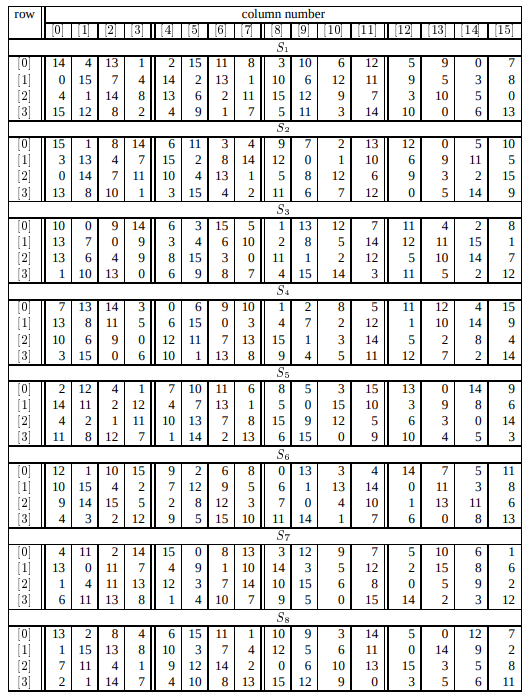
\includegraphics[scale=0.79]{Images/L_5-6/Des_Sbox.png}
\newpage

\subsection{Permutation :}

$P : \{0,1\}^{32} \rightarrow \{0,1\}^{32}$\\
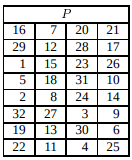
\includegraphics[scale=1.5]{Images/L_5-6/Des_Permutation.png}\\
$P(x_1\ x_2\ x_3\ .\ .\ .\ .\ x_32)\ =\ (x_{16}\ x_{7} .\ .\ .\ .\ x_{22}\ x_{11}\ x_4\ x_{25})$

\subsection{Des summary:}
\begin{enumerate}
    \item 16 rounds
    \item 64 bit block size
    \item key size of 64 bits
    \item IP and $IP^{-1}$
    \item Round function 
    \item Key scheduling algorithm
\end{enumerate}

\newpage
\section{Key scheduling algorithm DES:}

\textbf{Input :} 64 bit key k.

\textbf{Output :} 16 round keys.

\begin{enumerate}
    \item Define $V_i,\ 1 \le i \le 16\\$
    if i $\epsilon$ {1,2,9,16}\\
    {$V_i=1$}\\
    else $V_i = 2$
    \item Discard 8 parity bits from k.
    \item $T = PC_1(\Tilde{k})\quad PC_1 : \{0,1\}^{56} \rightarrow \{0,1\}^{56} $
    \item $(C_0,D_0)=T \quad Where\ C_0 \text{ is of 28 bit and } D_0 \text{ is of 28 bit.}$
    \item for i = 1 to 16\\
    $C_i = (C_{i-1} \hookleftarrow v_i)$\\
    $D_i = (D_{i-1} \hookleftarrow v_i)$\\
    
    $\begin{aligned}
    K_i = & PC_2 (C_i,D_i)\\
    & PC_2 : \{0,1\}^{56} \rightarrow \{0,1\}^{48}    
    \end{aligned}$
    \item Round key = $k_1\ k_2\ k_3\ k_4 \ .\ .\ .\ .\ k_{16}$\\\\
    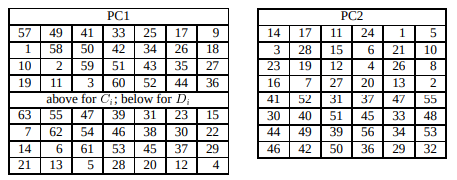
\includegraphics[scale=1.4]{Images/L_5-6/DES PC_1-PC_2.png}\\
    
\end{enumerate}
%%%%%%%%%%%%%%%%%%%%%%%%%%%%%%%%%%%%%%%%%%%%%%%%%%%%%%%%%%%%%%%%%%%%%
\end{document}